\documentclass[a4paper,12pt]{article}     %页面大小和字体大小
\usepackage{ctex}
\usepackage{geometry}
\usepackage{mathptmx}
\usepackage{amsmath}
\usepackage{graphicx}
\usepackage[T1]{fontenc}
\geometry{left=2.0cm, right=2.0cm, top=3.0cm, bottom=3.0cm}   %页边距
\linespread{1.5}      %行距

\begin{document}

\begin{center}   %居中设置
孟澍 \ 3210101819
\end{center}

\noindent %顶格(不缩进)
\textbf{2.40}\\
a. \ \verb|0 10000000 00000000000000000000000| is $+1.0 * 2^{128-127} = +2.$\\
b. \ \verb|1 10000011 00010000000000000000000| is $-1.0001 * 2^{131-127} = -17.$\\
c. \ \verb|0 11111111 00000000000000000000000| is positive infinity.\\
d. \ \verb|1 10000000 10010000000000000000000| = $-1.1001 * 2^{128-127} = -3.125.$\\

~\\
\textbf{2.43}\\
a. \ Hello!\\
b. \ hELLO!\\
c. \ Computers!\\
d. \ LC-2\\

~\\
\textbf{3.6}\\
\begin{tabular}{c c|c c c}
  \hline
  A & B & C & D & E \\
  \hline
  1 & 1 & 0 & 0 & 1 \\
  1 & 0 & 0 & 1 & 0 \\
  0 & 1 & 1 & 0 & 0 \\
  0 & 0 & 1 & 1 & 0 \\
  \hline
\end{tabular}

~\\
\textbf{3.20}\\
It will have one output line and four select lines.\\

\newpage
\textbf{3.23}\\
~\\
a. \
\begin{tabular}{c c c c | c}
  \hline
  A & B & C & D & Z \\
  \hline
  1 & 1 & 1 & 1 & 1 \\
  1 & 1 & 1 & 0 & 0 \\
  1 & 1 & 0 & 1 & 0 \\
  1 & 1 & 0 & 0 & 1 \\
  1 & 0 & 1 & 1 & 1 \\
  1 & 0 & 1 & 0 & 0 \\
  1 & 0 & 0 & 1 & 0 \\
  1 & 0 & 0 & 0 & 0 \\
  0 & 1 & 1 & 1 & 1 \\
  0 & 1 & 1 & 0 & 1 \\
  0 & 1 & 0 & 1 & 0 \\
  0 & 1 & 0 & 0 & 1 \\
  0 & 0 & 1 & 1 & 0 \\
  0 & 0 & 1 & 0 & 0 \\
  0 & 0 & 0 & 1 & 1 \\
  0 & 0 & 0 & 0 & 0 \\
  \hline
\end{tabular}\\

\newpage
b. \ \begin{figure}[h] 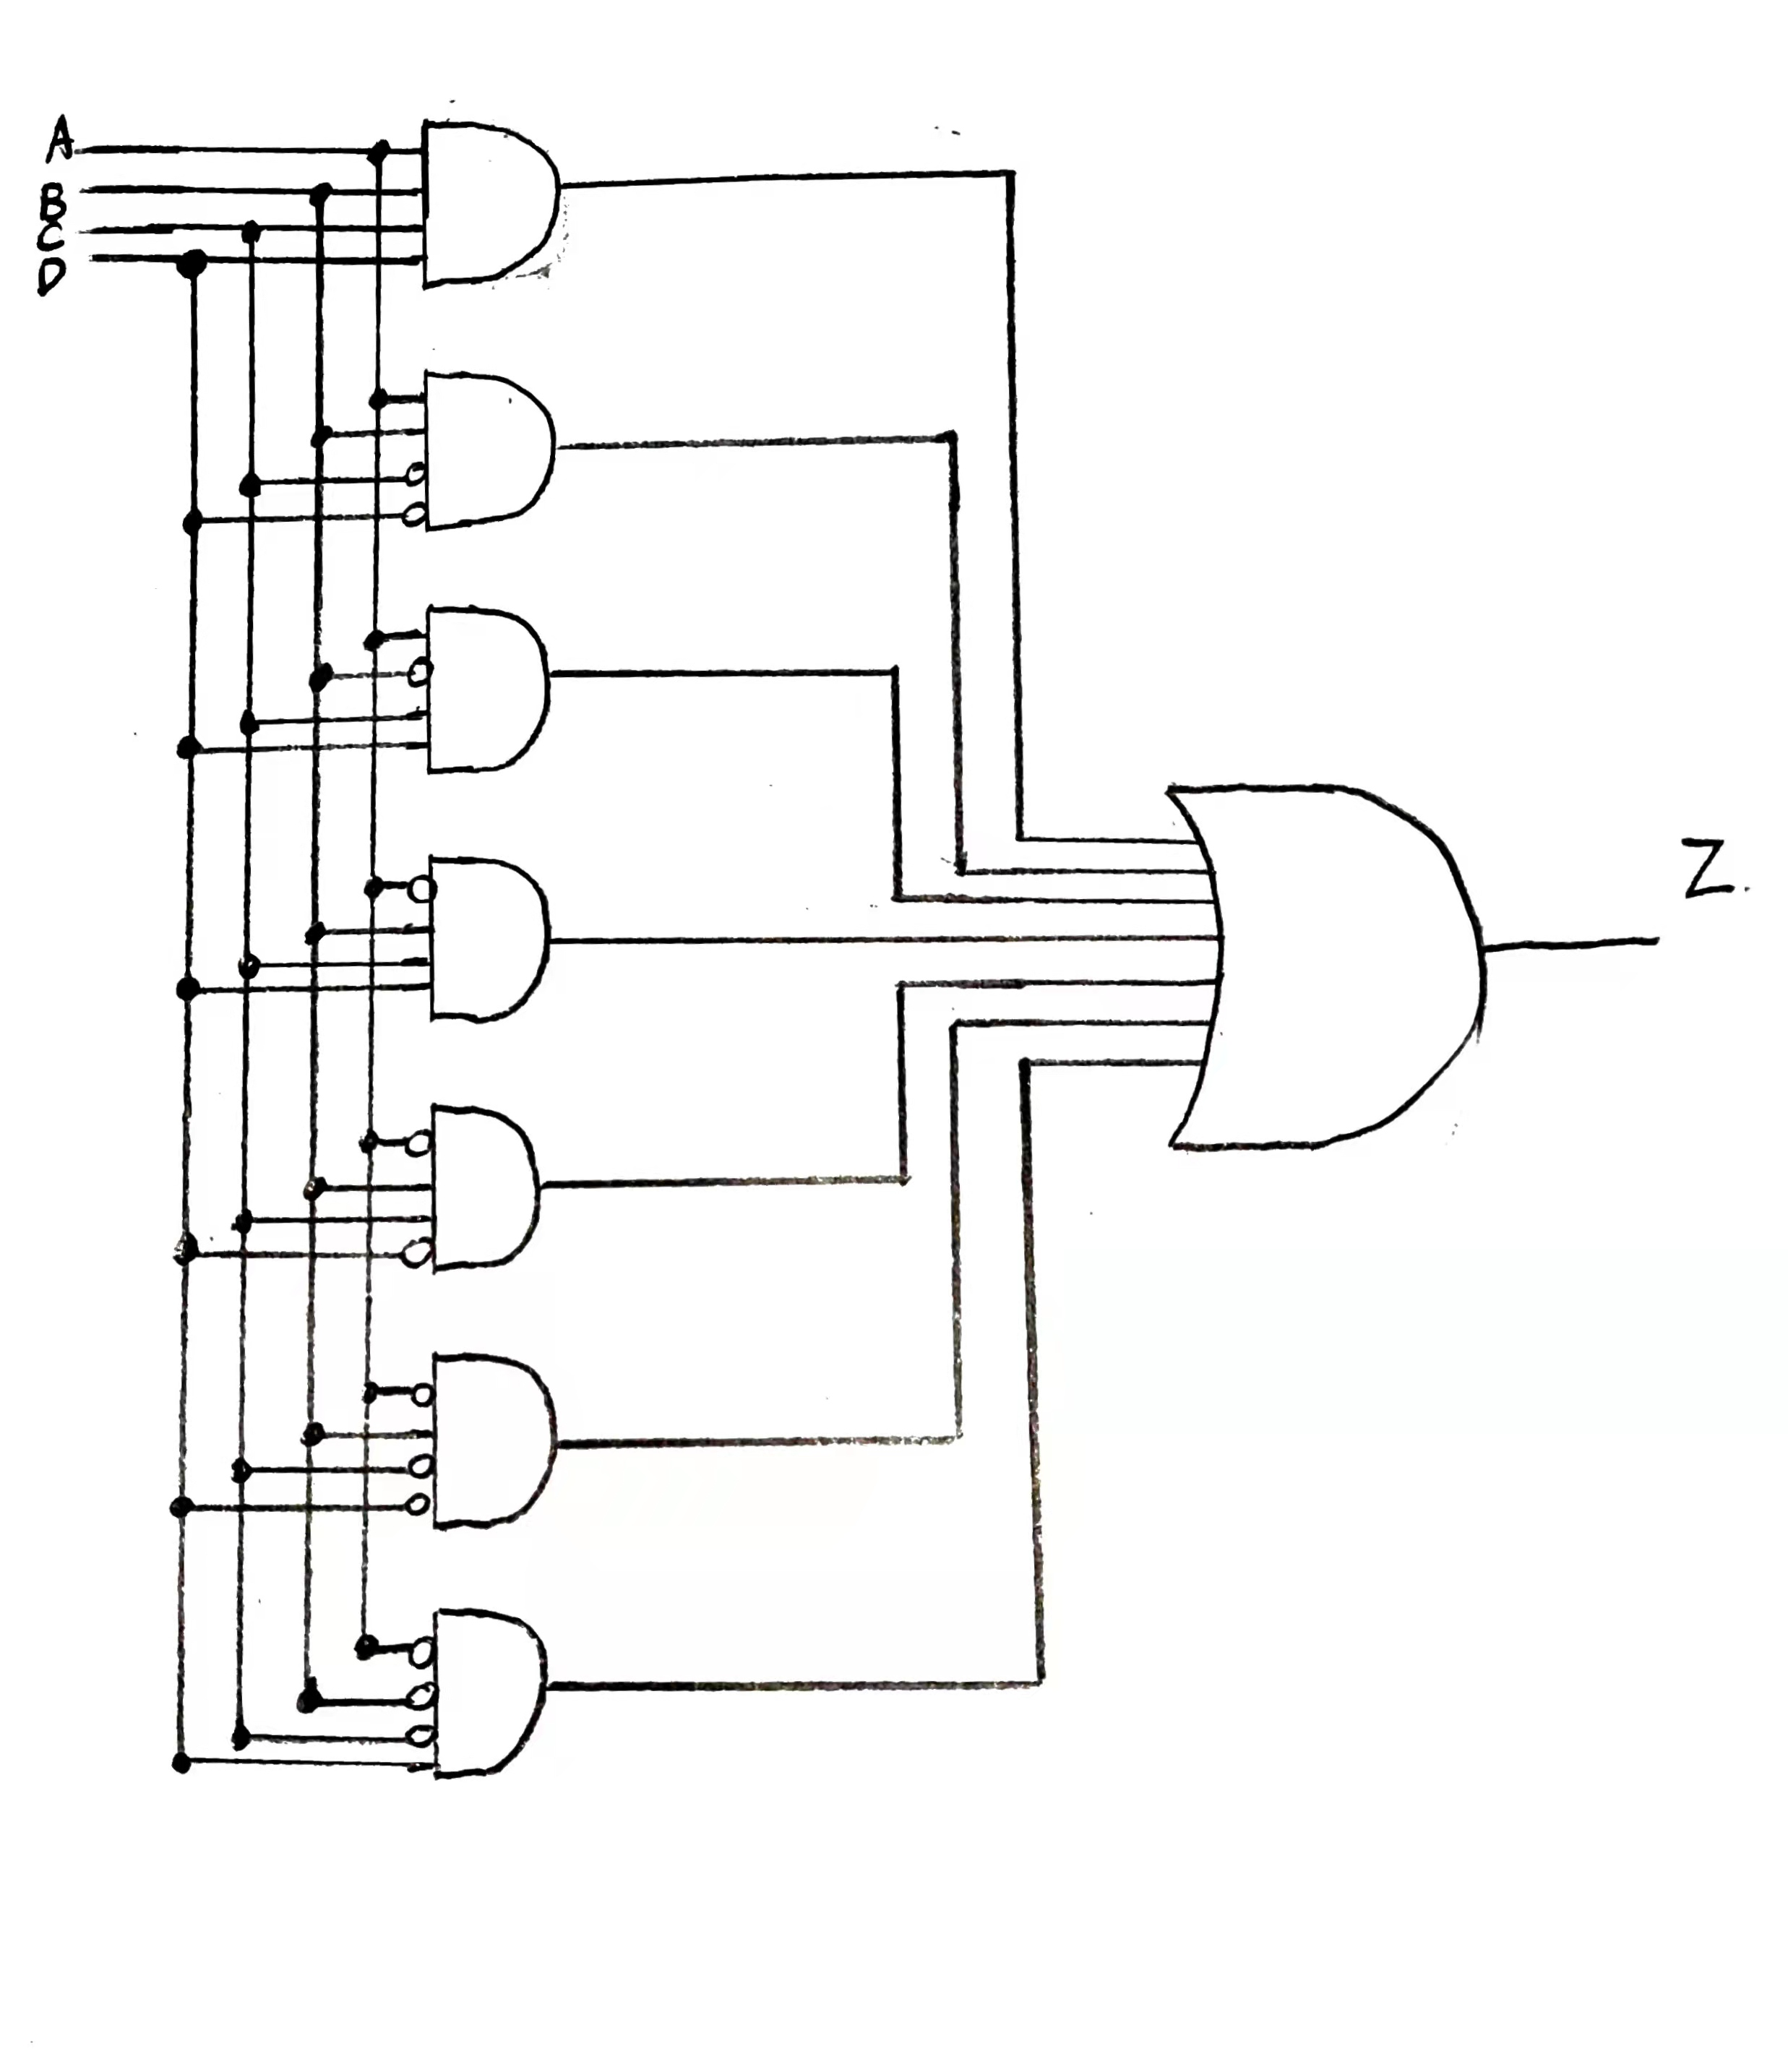
\includegraphics[width = 0.5\textwidth]{fig/fig1.jpeg} \end{figure}\\

\newpage
\textbf{3.26}\\
\begin{figure}[h] 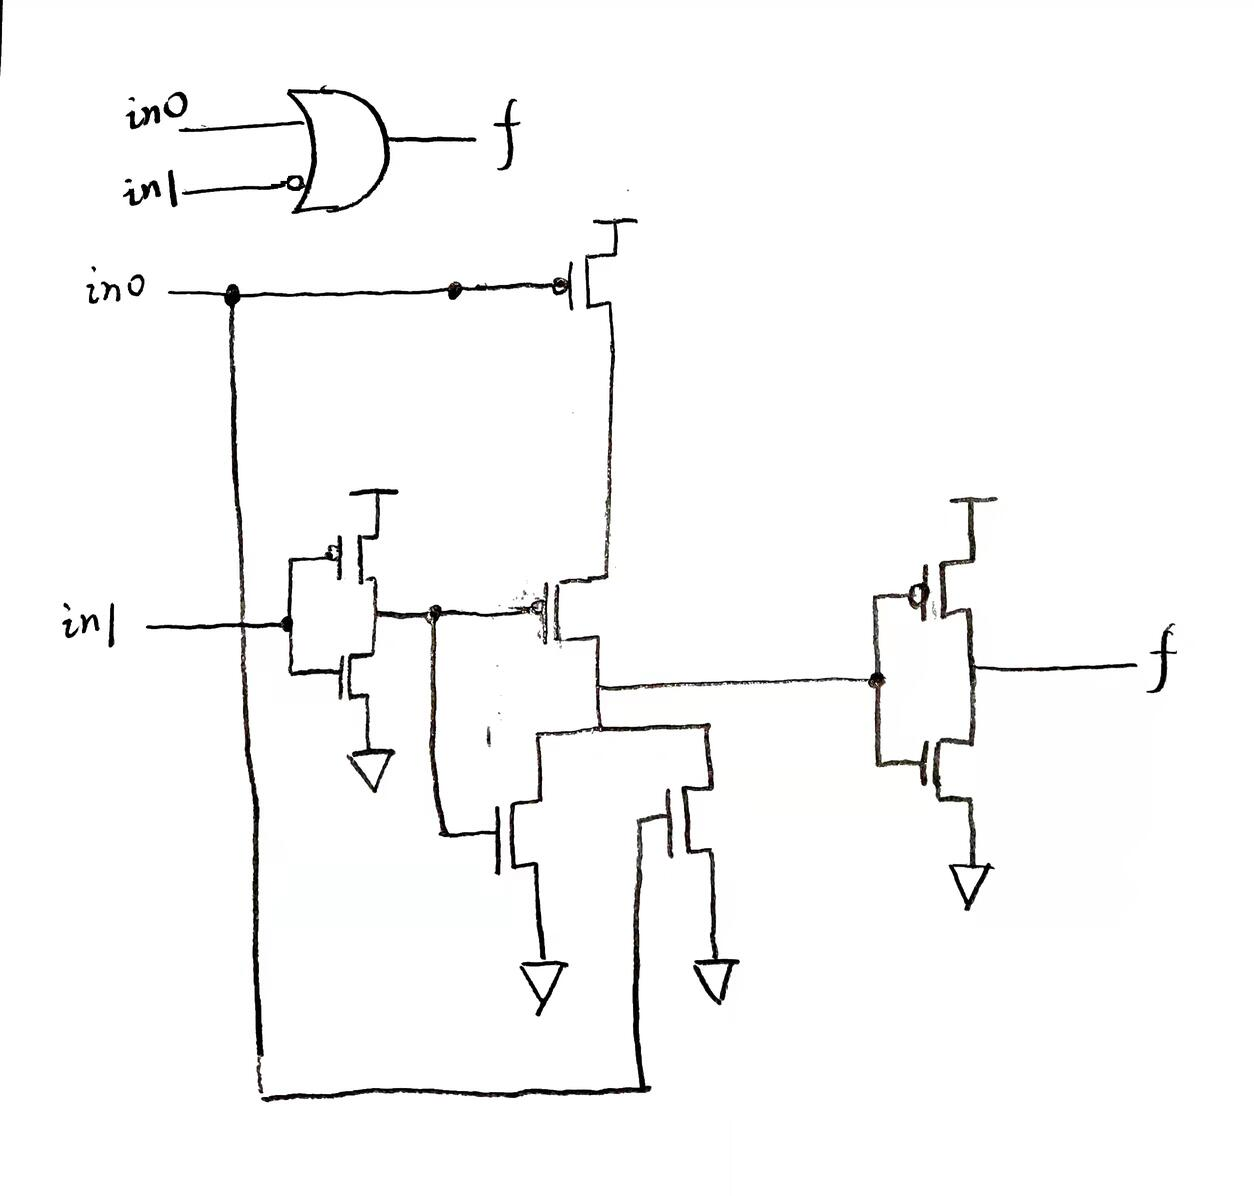
\includegraphics[width = 0.5\textwidth]{fig/fig2.jpeg} \end{figure}\\

\textbf{3.30}\\
a. \ When X = 0, the output is A + B. When X = 1, the output is A + C.\\
b. \ \begin{figure}[h] 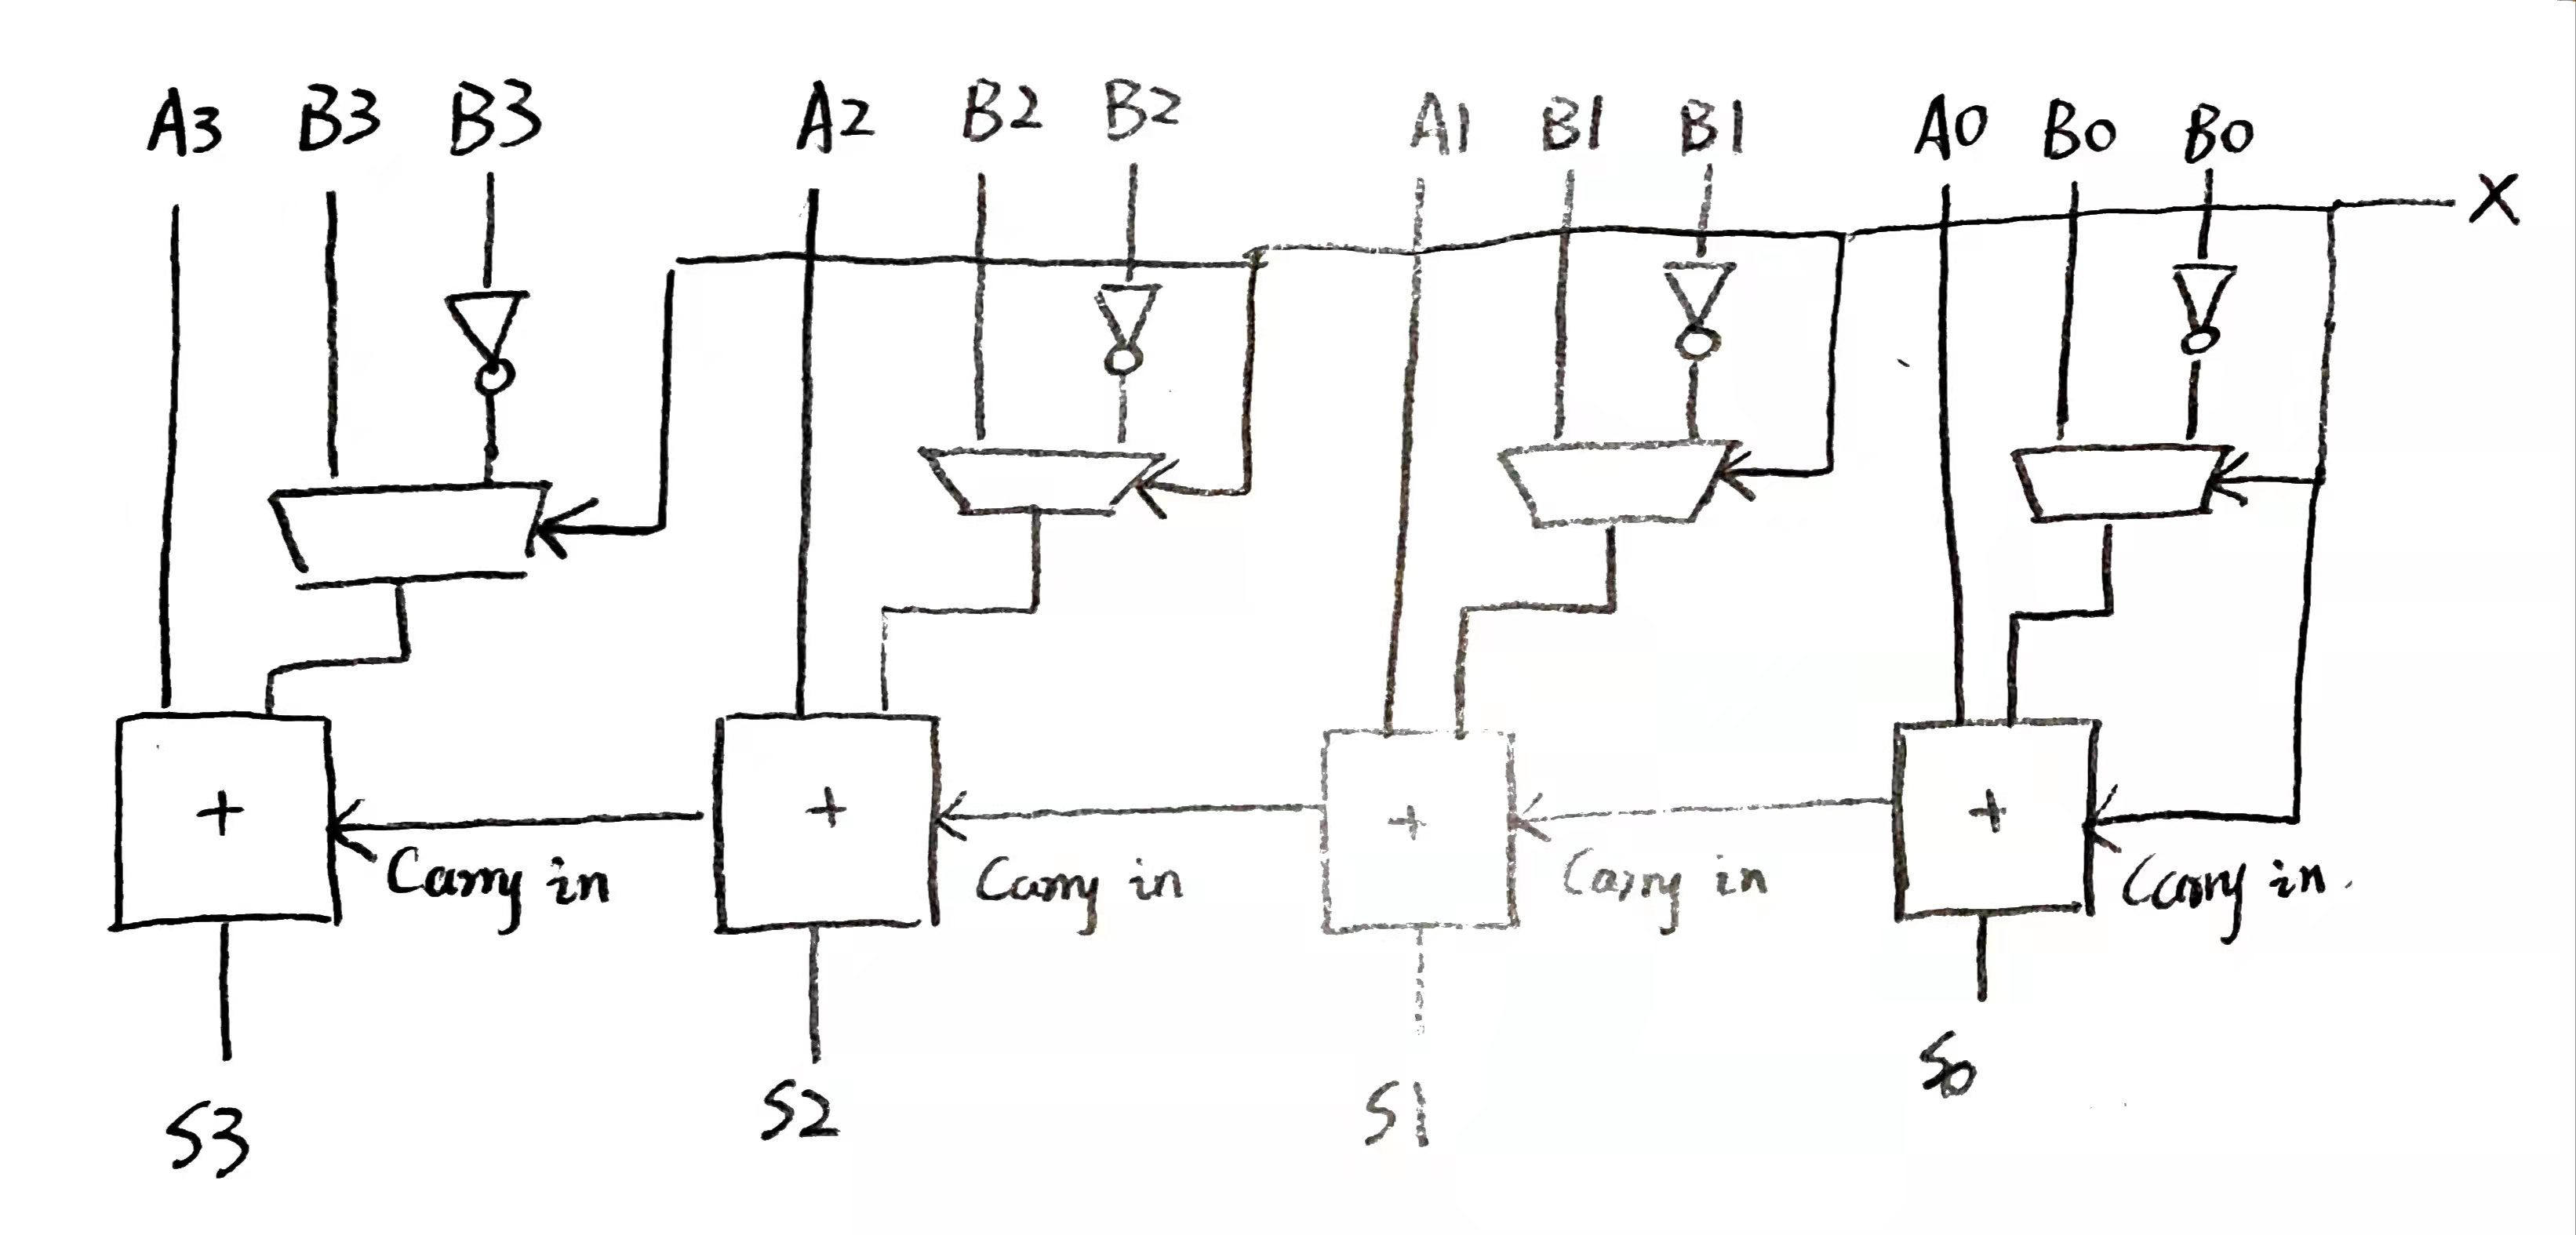
\includegraphics[width = 0.9\textwidth]{fig/fig3.jpeg} \end{figure}

\newpage
\textbf{3.36}\\
~\\
a. \
\begin{tabular}{c c|c c c}
  \hline
  A & B & G & E & L \\
  \hline
  0 & 0 & 0 & 1 & 0 \\
  0 & 1 & 0 & 0 & 1 \\
  1 & 0 & 1 & 0 & 0 \\
  1 & 1 & 0 & 1 & 0 \\
  \hline
\end{tabular}\\

b. \ \begin{figure}[h] 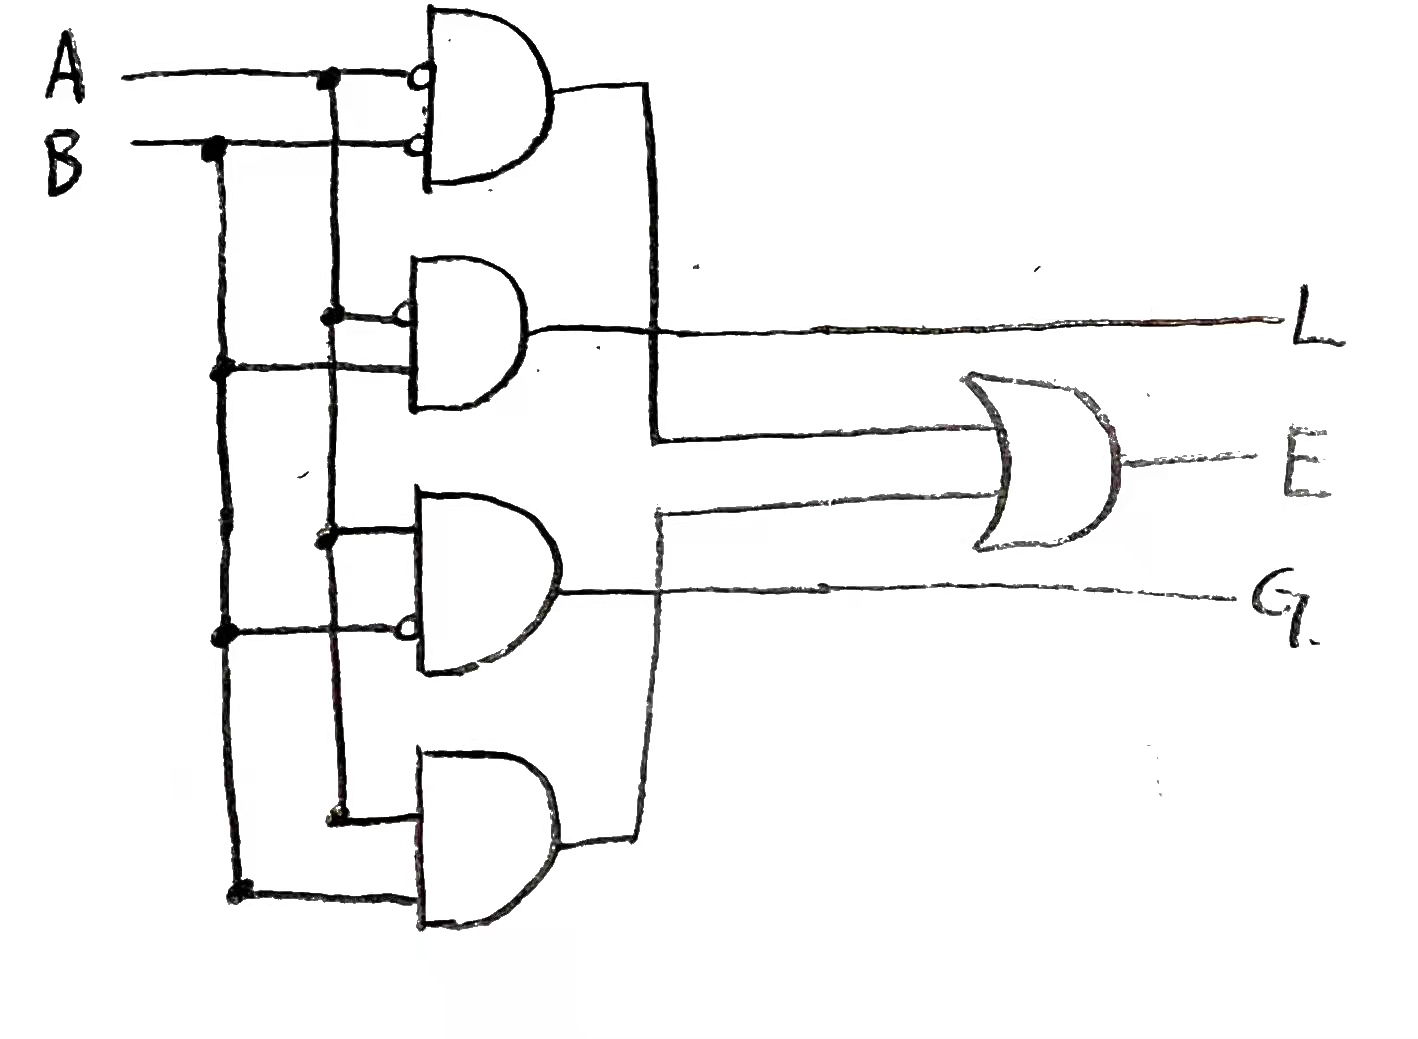
\includegraphics[width = 0.4\textwidth]{fig/fig4.jpeg} \end{figure}\\

c. \ \begin{figure}[h] 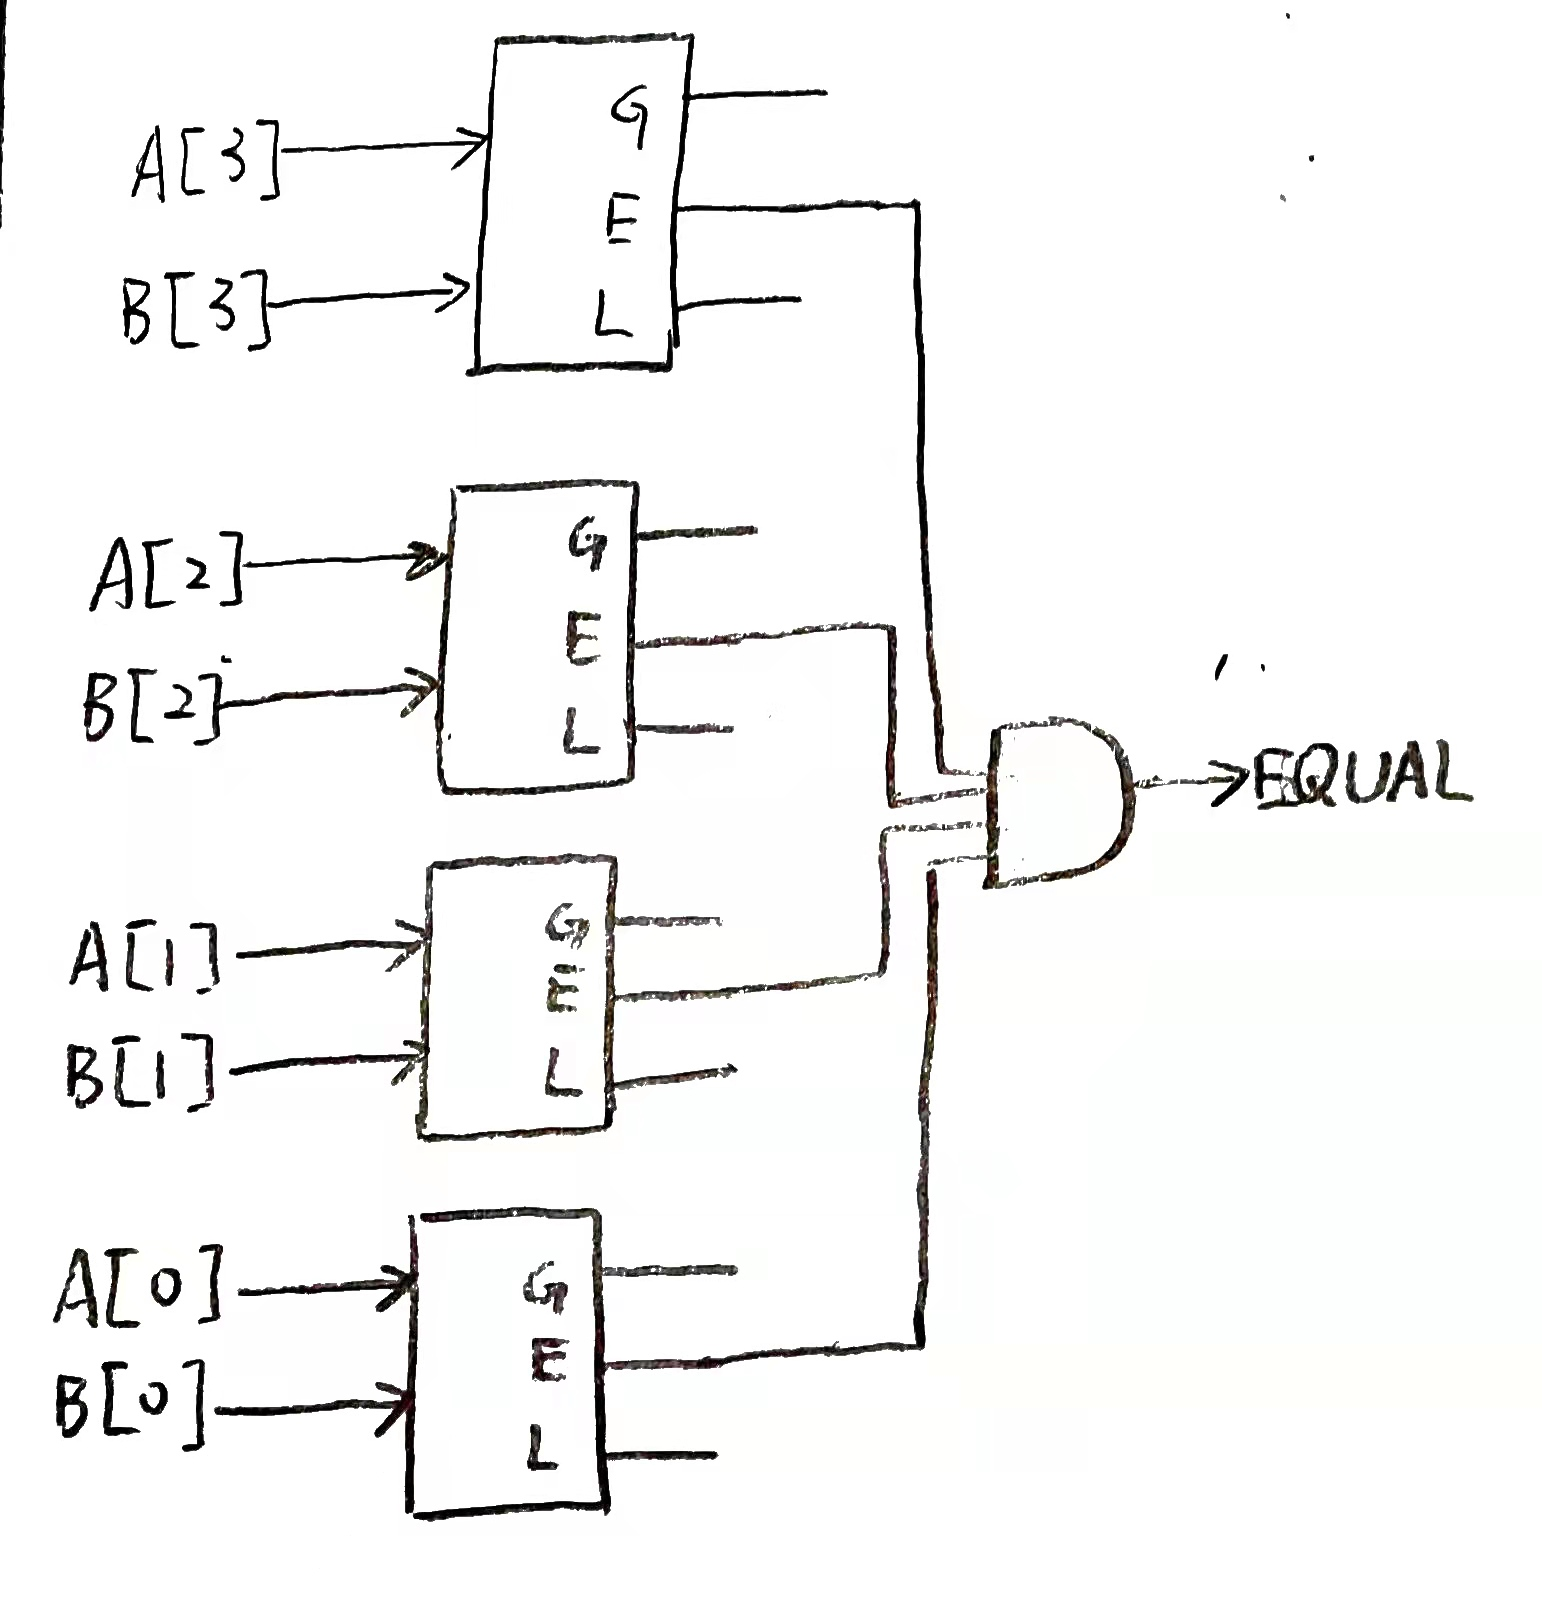
\includegraphics[width = 0.5\textwidth]{fig/fig5.jpeg} \end{figure}

\end{document}